\section{Original prototype}
\label{original}
\begin{comment}


\begin{figure*}[]
	\centering	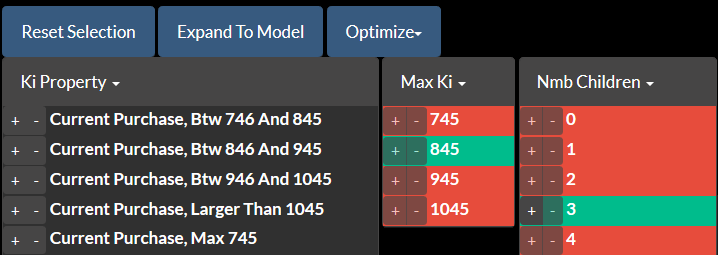
\includegraphics[angle=0,width = 0.6\linewidth]{img/oldscreen_joost.png} %, trim={2.5cm 21,7cm 2,2cm 2,0cm}, clip]
	\caption{Propagation in the original prototype.}
	\label{fig:old}
\end{figure*}
\end{comment}

At the start of the case study the notary's application requirements were rather vague.
The most important concern was to use the obtained information in an intelligent way, i.e., use the information instantly to derive conclusions.
Because of this we opted for the use of the earlier developed \textit{automatic configuration} interface that is available on the \idp homepage \cite{idphome}.
As the use of it is independent of the domain described in the vocabulary and theory in the knowledge base, this was an easy way to create a first visual prototype to solicit further application requirements from the notary.
%Figure \ref{fig:old} shows a screenshot of the original prototype that was developed in \cite{ruleml/DeryckHVV18} using the technology from \cite{ruleml/DassevilleJJVD16}. The interface allows to construct a partial interpretation: the ``$+$'' serves to assign a unique value to a constant, while the ``$-$'' removes the corresponding value from the domain of the constant.
%Applying propagation then leads to a more precise interpretation $\ci^{prop}$. 
For each propagated atom the corresponding box is colored green if the atom is true in $\ci^{prop}$, and red if it is false. In addition, the user may also invoke model expansion to complete the current partial interpretation into some total model, and optimization to complete it into the model expansion that minimizes the duties that need to be paid. 
%The notary office found the propagation and optimization inferences quite useful but did not see much use for model expansion.

%provides a user the possibility to construct an implicit structure by assigning truth values to all atoms over the modelled vocabulary by clicking $+$ (meaning: true) or $-$(meaning: false).
%As a result, the atom is highlighted in green resp. red.

%The development and characteristics of the original interactive decision enactment system (\ides) were described in \cite{Ingmar}, and its application in the registration duty domain in \cite{ruleml/DeryckHVV18}.
\begin{comment}

At the start of the case study the notary's application requirements were rather vague.
The most important concern was to use the obtained information in an intelligent way, i.e., use the information instantly to derive conclusions.
Because of this we opted for the use of the earlier developed \textit{automatic configuration} interface that is available on the \idp homepage \cite{idphome}.
As the use of the \ides~is independent of the domain described in the vocabulary and theory in the knowledge base, this was an easy way to create a first visual prototype to solicit further application requirements from the notary.
\end{comment}
%The interface provides a user the possibility to construct an implicit structure by assigning truth values to all atoms over the modelled vocabulary by clicking $+$ (meaning: true) or $-$(meaning: false).
%As a result, the atom is highlighted in green resp. red.
%Figure \ref{fig:old} shows a screenshot of this interface.



%The inferences performed by the original \ides are propagation, optimization and model expansion.

%\paragraph{Propagation}
%After the user has chosen some atoms' truth values, the consequences of these choices are automatically calculated by \idp's propagation inference. 
%The output of this inference is a set of atoms that hold in all models to the current set of choices. The resulting true atoms are highlighted in green, the false ones in red.
%This allows the user to see the impact of his selections at a glance.
%For experienced users, this is helpful in determining which other parts of information should be requested.
%\jo{last sentence needed?}

%In Figure \ref{fig:old}, the number of children is chosen to be three by assigning the corresponding atom to true, and from this follows that the maximum \textit{kadastral income} (KI) is 845.
%Both are highlighted in green, while the red atoms represent now impossible choices.

%\paragraph{Optimization}
%In complex situations, multiple combinations of \textit{abattement} and registration type might be possible, each leading to an other duty to be paid.
%Typically buyers would prefer to use the option that minimizes this amount, which is calculated by using the optimization inference in the interface.
%For this functionality, we added the following objective function:
%\[
%(BaseAmount * ApplicableRate)- TotalPortability
%\]

%\paragraph{Model expansion}
%The expansion of an incomplete structure to a model that satisfies the theory can be useful for training or validation purposes.
%E.g., if the notary wants to explain to a client in which cases he would be entitled to the rate for social dwellings, he might do this by enforcing the atom assignment $HasRegistrationType=socialDwelling \mapsto \true$ and generating a model.
%\jo{is dit het juiste atoom? Ik ben niet meer zeker van m'n aanpassing...}
